\chapter{Theoretical background and related work}\label{ch:related}
\thispagestyle{pagestyle}

This chapter creates the state-of-the-art for this thesis. The minimum quantum-computing background comes first, followed by the classical image and edge metrics used for scoring. From there the chapter surveys quantum image representations and edge detectors, explains the NISQ constraints and the multi-controlled synthesis choice at the heart of the study, and then positions this work against the literature~\cite{NielsenChuang2010,Ruan2021OpportunitiesChallenges,Wang2022ReviewQIP}.

\section{Quantum computing essentials}

\subsection{Classical bits versus quantum states}
Ordinary computers store information in \emph{bits}. A bit is the smallest unit of data and is always in exactly one of two states, written $0$ or $1$. Every number, image, or program a classical computer handles is ultimately a long string of such bits.

A quantum computer replaces the bit with a \emph{qubit} (quantum bit). The two definite values $0$ and $1$ still exist and are written $\ket{0}$ and $\ket{1}$; the angled-bracket notation $\ket{\cdot}$ is the standard way to label a quantum state and can be read simply as ``the state.'' Unlike a bit, though, a qubit may sit in a blend of both values at once, at least until it is read out. Such a blend is written
\begin{equation}
\ket{\psi} = \alpha\ket{0} + \beta\ket{1}, \qquad |\alpha|^2 + |\beta|^2 = 1 .
\end{equation}
Here $\ket{\psi}$ denotes the qubit's state, and the two coefficients $\alpha$ and $\beta$ (called \emph{amplitudes}) say ``how much'' of $\ket{0}$ and of $\ket{1}$ the blend contains. The amplitudes are complex numbers rather than ordinary fractions, and that is what later lets contributions add up or cancel, as overlapping waves do. Geometrically, a qubit state is just a unit-length arrow (a \emph{unit vector}) in a two-dimensional space whose two reference directions are $\ket{0}$ and $\ket{1}$.

Reading a qubit is called \emph{measurement}, and it never returns the blend itself: it always yields a single classical answer, either $0$ or $1$. The probability of each outcome is fixed by the amplitudes through the squared magnitudes $|\alpha|^2$ and $|\beta|^2$, and these two probabilities must add to one, which is the content of the constraint $|\alpha|^2 + |\beta|^2 = 1$. A qubit poised between both values is said to be in \emph{superposition}; the act of measuring forces it to ``pick'' one value and discards the rest of the blend, a phenomenon often called \emph{collapse}.

Superposition becomes powerful when qubits are combined. With $n$ classical bits a register holds one of $2^n$ possible patterns at a time (for example, three bits give the eight patterns $000,001,\dots,111$). With $n$ qubits the state can be a weighted blend of all $2^n$ patterns simultaneously: formally, $n$-qubit pure states live in a $2^n$-dimensional space spanned by the basis labels $\ket{x_{n-1}}\cdots\ket{x_0}$, where each $x_i$ is one bit of the pattern. This exponential room is the resource quantum algorithms try to exploit. A single measurement, however, still returns only one of those $2^n$ patterns, so a useful algorithm must shape the amplitudes through \emph{interference}, in which wrong answers cancel and right answers reinforce, so that the desired pattern is the one most likely to appear~\cite{NielsenChuang2010}.

\subsection{Gates, circuits, and transpilation}
Between measurements a closed system evolves \emph{unitarily}: $\ket{\psi}\mapsto U\ket{\psi}$. The single-qubit gates used here are the Pauli-$X$ bit-flip (\Cref{fig:tikz-paulix}), the Hadamard $H$ that creates equal superpositions (\Cref{fig:tikz-hadamard}), and the $y$-rotation $R_y(\theta)=\exp(-\mathrm{i}\theta Y/2)$ that FRQI uses to write grayscale angles (\Cref{fig:tikz-ry}). The two-qubit CNOT (CX) gate is the main bottleneck on superconducting hardware because it is slower and noisier than single-qubit pulses~\cite{Geng2023ImprovedFRQI}.

\begin{figure}[htbp]
\centering
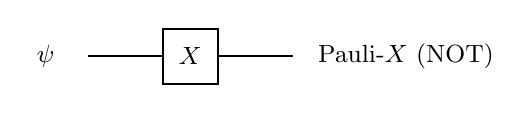
\begin{tikzpicture}[scale=1.0, every node/.style={font=\small}]
  \node[left] at (-0.3,0.5) {$\ket{\psi}$};
  \draw[thick] (0,0.5) -- (0.95,0.5);
  \draw[thick] (1.65,0.5) -- (2.6,0.5);
  \draw[thick] (0.95,0.15) rectangle (1.65,0.85);
  \node at (1.3,0.5) {$X$};
  \node[right] at (2.8,0.5) {Pauli-$X$ (NOT)};
\end{tikzpicture}
\caption{Symbolic Pauli-$X$ gate: the box applies $X$ to the qubit, flipping $\ket{0}\leftrightarrow\ket{1}$.}
\label{fig:tikz-paulix}
\end{figure}

\begin{figure}[htbp]
\centering
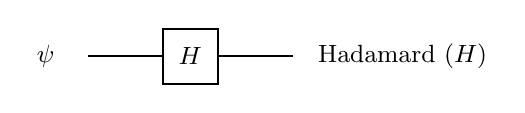
\begin{tikzpicture}[scale=1.0, every node/.style={font=\small}]
  \node[left] at (-0.3,0.5) {$\ket{\psi}$};
  \draw[thick] (0,0.5) -- (0.95,0.5);
  \draw[thick] (1.65,0.5) -- (2.6,0.5);
  \draw[thick] (0.95,0.15) rectangle (1.65,0.85);
  \node at (1.3,0.5) {$H$};
  \node[right] at (2.8,0.5) {Hadamard ($H$)};
\end{tikzpicture}
\caption{Symbolic Hadamard gate: the box applies $H$ to the qubit, sending the basis states $\ket{0}$ and $\ket{1}$ to equal superpositions.}
\label{fig:tikz-hadamard}
\end{figure}

\begin{figure}[htbp]
\centering
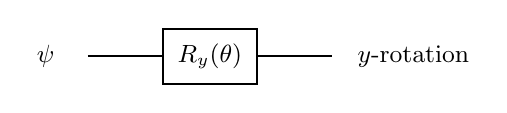
\begin{tikzpicture}[scale=1.0, every node/.style={font=\small}]
  \node[left] at (-0.3,0.5) {$\ket{\psi}$};
  \draw[thick] (0,0.5) -- (0.95,0.5);
  \draw[thick] (2.15,0.5) -- (3.1,0.5);
  \draw[thick] (0.95,0.15) rectangle (2.15,0.85);
  \node at (1.55,0.5) {$R_y(\theta)$};
  \node[right] at (3.3,0.5) {$y$-rotation};
\end{tikzpicture}
\caption{Symbolic $y$-rotation gate: the box applies $R_y(\theta)=\exp(-\mathrm{i}\theta Y/2)$, which FRQI uses to encode a grayscale intensity as a rotation angle on the color qubit.}
\label{fig:tikz-ry}
\end{figure}

A \emph{quantum circuit} is a sequence of gates on named qubits. Its \emph{depth} counts parallel time steps, and its \emph{CX count} measures two-qubit cost once the circuit is rewritten into a hardware-native gate set. Because a small gate set can approximate any unitary, compilers \emph{transpile} a logical circuit into native basis gates (here \texttt{cx}, \texttt{rz}, and \texttt{sx}) and optimize depth~\cite{NielsenChuang2010}. \Cref{fig:tikz-cnot} fixes the CNOT symbol used throughout.

\begin{figure}[htbp]
\centering
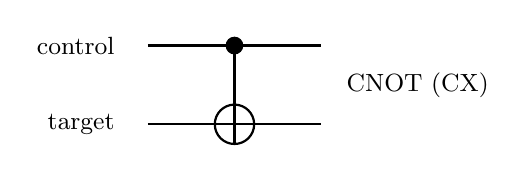
\begin{tikzpicture}[scale=1.0, every node/.style={font=\small}]
  \node[left] at (-0.3,1.5) {control};
  \node[left] at (-0.3,0.5) {target};
  \draw[thick] (0,1.5) -- (2.2,1.5);
  \draw[thick] (0,0.5) -- (0.85,0.5);
  \draw[thick] (1.35,0.5) -- (2.2,0.5);
  \filldraw (1.1,1.5) circle (3pt);
  \draw[thick] (1.1,1.5) -- (1.1,0.5);
  \draw[thick] (1.1,0.5) circle (0.25);
  \draw[thick] (0.85,0.5) -- (1.35,0.5);
  \draw[thick] (1.1,0.25) -- (1.1,0.75);
  \node[right] at (2.4,1.0) {$\mathrm{CNOT}$ (CX)};
\end{tikzpicture}
\caption{Symbolic CNOT gate: the filled circle marks the control qubit; the segment on the lower wire denotes $X$ on the target conditioned on control $\ket{1}$.}
\label{fig:tikz-cnot}
\end{figure}

\subsection{Measurement and end-of-circuit readout}
A quantum computation is only useful once its result is brought back into the ordinary, classical world, and the single operation that does this is \emph{measurement}. As introduced above, measuring a qubit forces it out of any blend and returns one definite bit, $0$ or $1$, with probabilities set by the amplitudes. Two practical consequences follow. First, a measurement is destructive: the blend is gone afterward, so a value cannot be ``peeked at'' and then reused. Second, one run reveals only one bit per qubit, not the underlying probabilities. To estimate those probabilities the same circuit is therefore prepared and measured many times (each repetition is called a \emph{shot}), and the fraction of runs that returned each pattern approximates its probability. The more shots, the closer this estimate. The collection of measured bit strings is the classical data every result in this thesis is computed from. (In \emph{density-matrix} mode the simulator instead tracks the full pre-measurement state and reports the ideal probabilities those shots would converge to, which removes sampling noise but is more memory-hungry.)

Where in a circuit should measurement happen? The \emph{principle of deferred measurement} states that measurements made in the middle of many algorithms can be pushed to the very end without changing the final statistics, provided the would-be measurement is replaced by a reversible (unitary) interaction with an extra helper qubit, called an \emph{ancilla}~\cite{NielsenChuang2010}. Intuitively, instead of reading a qubit early and acting on the classical outcome, the circuit ``writes'' that information onto an ancilla and keeps everything quantum until the final readout. This keeps the noiseless, reversible part of the computation cleanly separated from the one irreversible, classical step at the end, which is why every pipeline here ends in a single computational-basis readout.

This separation matters for FRQI, where the color qubit stores each pixel's grayscale value in its amplitude, so the reconstructed image depends directly on how reliably that qubit is read. Two very different error sources both blur the result, and they should not be conflated. \emph{Gate noise} corrupts the quantum state itself while the circuit runs, as imperfect pulses and decoherence nudge the true state away from the intended one. \emph{Readout (assignment) error} happens only at the measurement step: the state may be correct, yet a true $0$ is occasionally reported as $1$ and vice versa. These mislabelling rates can be summarized in a small \emph{confusion matrix} whose entries are the probabilities ``reported value given true value.'' The mitigation step discussed later inverts this matrix to undo the mislabelling; crucially it only relabels classical outcomes and leaves the quantum edge-detection (QHED) stage untouched~\cite{Mu2025GuidedImageFiltering}. Keeping gate noise and readout error apart prevents one from being mistaken for the other when interpreting results. \Cref{fig:frqi-flow} sketches the FRQI data flow that ties these pieces together.

\begin{figure}[htbp]
\centering
\begin{tikzpicture}[
  box/.style={draw, rounded corners=2pt, minimum width=3.4cm, minimum height=0.9cm, align=center, font=\small},
  arr/.style={-{Latex[length=2.2mm]}, thick}
]
  \node[box] (pos) {Position register\\$m$ qubits (addresses)};
  \node[box, below=1.1cm of pos] (col) {Color qubit\\$R_y(\theta_p)$ when $\ket{p}$ matches};
  \node[box, below=1.1cm of col] (meas) {Measurement / decoding\\intensities from $c$};
  \draw[arr] (pos) -- node[midway, right=1mm, font=\scriptsize, align=left] {multi-controlled\\steering} (col);
  \draw[arr] (col) -- node[midway, right=1mm, font=\scriptsize, align=left] {shots /\\density matrix} (meas);
\end{tikzpicture}
\caption{FRQI data flow: addresses live in the position register; each pixel angle is applied conditional on address comparisons; classical readout reconstructs an image.}
\label{fig:frqi-flow}
\end{figure}

\subsection{The NISQ setting}
The quantum computers available today are not the flawless, error-corrected machines of theory. The term \emph{noisy intermediate-scale quantum} (NISQ) captures this reality, and its three words name the three constraints. \emph{Noisy} means every operation has a chance of going wrong. \emph{Intermediate-scale} means the machines have only tens to a few hundred qubits, enough to be interesting but too few to spare any for full error correction. \emph{Quantum} simply marks that they still exploit superposition and entanglement~\cite{Preskill2018NISQ,Geng2022HybridNISQEdge}.

Several concrete limitations sit behind that label. The qubit count is small, so circuits cannot afford many helper qubits. \emph{Connectivity} is limited: a two-qubit gate can only act on physically adjacent qubits, so interacting two distant qubits forces the compiler to insert extra swap operations, each adding more error-prone gates. \emph{Coherence times}, written $T_1$ and $T_2$, are how long a qubit keeps its information before it decays ($T_1$ is roughly how long a $\ket{1}$ survives before relaxing to $\ket{0}$, and $T_2$ how long a superposition keeps its phase), so any circuit must finish well within these windows or its data simply fades. \emph{Calibration drift} means the fine-tuning of the gates slowly goes stale over hours, and \emph{readout errors} are the measurement mistakes described above.

These limits hurt quantum image processing twice over. First, just \emph{preparing} a data-dependent state such as FRQI already costs many multi-controlled operations, which is exactly where gate noise and depth pile up. Second, whatever runs afterwards (here the QHED edge detector) assumes the prepared state is close to ideal, so errors from preparation propagate straight into the result. This double exposure is why surveys agree that near-term progress comes from matching algorithms to real hardware constraints, rather than from chasing the best asymptotic complexity on paper~\cite{Ruan2021OpportunitiesChallenges,Farooq2025SystematicReview}.

\subsection{Noise models and simulation cost}
To predict how a circuit behaves on imperfect hardware without owning a quantum computer, the noise is imitated in software. The simplest useful model is the \emph{depolarizing channel}, applied after each single- and two-qubit gate (Qiskit Aer's density-matrix backend supports this directly). The idea is easy to picture. After a gate, with some small probability $p$ the qubit's information is thrown away and replaced by complete randomness (the \emph{maximally mixed state}, which keeps no useful structure), while with probability $1-p$ the qubit is untouched. A single gate with tiny $p$ barely matters, but a deep circuit applies thousands of gates, and these small chances accumulate, so the final state drifts steadily toward randomness. This gradual loss of quantum structure is what the terms \emph{coherence} and \emph{purity} measure, and it is the core reason deep circuits fail on real devices.

Simulating this faithfully is expensive, and the cost depends on what the simulator must store. A noiseless run can use \emph{statevector} simulation, which keeps the $2^n$ complex amplitudes of an $n$-qubit pure state. Once noise mixes the state, a pure-state description no longer suffices: the simulator must switch to a \emph{density matrix}, an $n$-qubit state's full description as a $2^n\times 2^n$ table, i.e.\ $4^n$ real numbers. That squares the memory: going from $2^n$ to $4^n$ means each extra qubit roughly quadruples the storage instead of doubling it. Near $n\approx 16$ this exhausts RAM that is currently available on the budget machine available on the market.~\cite{NielsenChuang2010}.

Depolarizing noise is a deliberate simplification. The most general physically valid noise process is a completely positive, trace-preserving map, which can always be written as a short list of matrices (a \emph{Kraus} decomposition); the depolarizing channel is just one easy-to-specify member of that family, chosen here because it needs only a single number $p$ per gate type and plugs cleanly into Qiskit~\cite{NielsenChuang2010}. Real hardware also suffers slower, time-correlated (non-Markovian) effects such as calibration drift and $1/f$ flux noise, which can dominate in practice but are deliberately left outside the simulator configuration used here.

\subsection{Readout error and classical post-processing}
The final readout step is itself imperfect: the hardware that decides whether a qubit is $\ket{0}$ or $\ket{1}$ occasionally reports the wrong value. These mistakes are systematic rather than random, so they can be measured once and then corrected. The recipe is to prepare known inputs (a definite $0$, then a definite $1$) many times and record how often each is read back correctly. For one qubit this gives a $2\times 2$ table of ``reported given true'' probabilities, the \emph{confusion matrix} $A$. If $\mathbf{p}$ is the vector of true outcome probabilities, the frequencies actually observed are the distorted version $\mathbf{p}'\approx A\mathbf{p}$.

Correcting the bias is then a matter of running this relationship backwards. Since $A$ is known, multiplying the observed frequencies by its inverse $A^{-1}$ recovers an estimate of the true probabilities $\mathbf{p}$; this undo step is the \emph{mitigation}~\cite{Mu2025GuidedImageFiltering}. The correction matters for FRQI specifically because grayscale lives in the color qubit's outcome statistics, so a biased readout shifts the reconstructed pixel intensities even when the quantum state before measurement was perfectly correct.

One numerical caution applies. When the device is very noisy, $A$ is close to having no inverse at all (\emph{near-singular}), and a raw inversion then wildly amplifies the ordinary statistical scatter of finitely many shots. The standard remedy is \emph{Tikhonov regularization}, $(A^\top A + \lambda I)^{-1}A^\top$, where a small term $\lambda$ keeps the inversion numerically stable at the price of a slight, controlled bias, a deliberate trade of accuracy for steadiness. The demonstration slice here uses conservative (small) regularization~\cite{Mu2025GuidedImageFiltering}.

\section{Classical images, edges, and quality metrics}
\label{sec:classical-metrics}
Because the quantum pipelines in this thesis are ultimately judged as ordinary pictures, the comparison relies on classical image concepts, which this section sets out plainly. A digital grayscale image is simply a grid (a matrix) of numbers: each cell is one \emph{pixel}, and its number is the brightness at that spot. The brightness is usually stored in eight bits, giving $256$ levels from $0$ (black) to $255$ (white). An \emph{edge} is a place where brightness changes sharply between neighbouring pixels, for instance the outline of an object against its background, and \emph{edge detection} is any procedure that turns an image into a map highlighting those transitions. Classical edge detectors are small sliding filters such as Sobel, Prewitt, or Kirsch, and their output is then \emph{scored} against a trusted reference to say how good it is~\cite{Zhang2015QSobel,Zhou2019PrewittNEQR,Xu2020Kirsch}. Since the quantum methods here export bitmaps too, these same classical definitions stay the scoring interface even when the internal operation is not literally Sobel~\cite{Yao2017QHED}.

Scoring needs a number that says how close two images are. Let $I$ be the ground-truth (reference) image and $\hat{I}$ the reconstructed one, both $N\times N$ with $N_{\mathrm{pix}}=N^2$ pixels. The most direct measure, \emph{mean squared error}, simply looks at every pixel, takes the difference between the two images there, squares it (so over- and under-shoots both count as error and large misses are penalized more), and averages over all pixels:
\begin{equation}
\mathrm{MSE}(I,\hat{I}) = \frac{1}{N_{\mathrm{pix}}}\sum_{p=0}^{N_{\mathrm{pix}}-1}\bigl(I[p]-\hat{I}[p]\bigr)^2 .
\end{equation}
A smaller MSE means a closer match, and $0$ means identical. Raw MSE values are hard to interpret, so the \emph{peak signal-to-noise ratio} restates the same information on a logarithmic decibel scale, comparing the error to the largest possible intensity $L=255$ for eight-bit data:
\begin{equation}
\mathrm{PSNR}(I,\hat{I}) = 10\log_{10}\frac{L^2}{\mathrm{MSE}(I,\hat{I})}\quad(\mathrm{dB}).
\end{equation}
Here a \emph{higher} PSNR means a cleaner reconstruction (less error relative to full scale). Both MSE and PSNR, however, compare pixels one at a time and ignore how pixels relate to their neighbours, so they can rate a perceptually obvious distortion as mild. \emph{Structural similarity} (SSIM) addresses this by comparing small patches of the two images through three local factors, namely brightness (luminance), contrast, and structure (the pattern of variation), and combining them; this thesis uses the standard windowed variant from scikit-image. SSIM ranges over $[-1,1]$, where $1$ means the patches agree perfectly. Because edges are about contrast along contours, which is exactly what humans notice, SSIM is the structural proxy used when QHED output is compared to a Sobel reference~\cite{Chetia2021ImprovedSobelNEQR}.

It remains to define that reference. The discrete \emph{Sobel operator} is the classic way to find edges. Intuitively it estimates how fast brightness changes in the horizontal and vertical directions by sliding two small $3\times 3$ weight grids (\emph{kernels}) over the image; each kernel multiplies a pixel and its eight neighbours by fixed weights and sums them, producing a large response only where brightness rises steeply across that direction:
\begin{equation}
G_x = \begin{bmatrix}-1&0&+1\\-2&0&+2\\-1&0&+1\end{bmatrix},\qquad
G_y = \begin{bmatrix}-1&-2&-1\\0&0&0\\+1&+2&+1\end{bmatrix}.
\end{equation}
The left kernel $G_x$ reacts to left-to-right changes and the right one $G_y$ to top-to-bottom changes (note the positive and negative sides that subtract one neighbourhood from the opposite one). Combining both directions, the \emph{gradient magnitude} $\sqrt{(G_x*I)^2+(G_y*I)^2}$ (where $*$ denotes this sliding-and-summing operation, called convolution) gives a single edge-strength value per pixel, and the resulting edge map is what serves as the QHED reference. Prewitt and Kirsch masks just change the weights while keeping the same local-derivative idea~\cite{Zhou2019PrewittNEQR,Xu2020Kirsch}. Multi-scale and multi-direction variants exist because one fixed $3\times 3$ kernel is sensitive to noise and biased toward its two axes~\cite{Liu2022EightDirectionSobelNEQR}; quantum edge detectors inherit the same robustness questions and must ultimately be read against these classical references to stay interpretable~\cite{Fan2019SobelNEQR}.

\section{Quantum image representations}
Before an image can be processed on a quantum computer it must first be \emph{encoded} into a quantum state, which means the pixels of an ordinary picture are rewritten as amplitudes and qubits. Different encodings make different trade-offs between how many qubits are needed and how complicated the preparation circuit becomes, and that choice drives everything downstream. This section describes the two main families and why this thesis builds on FRQI.

\subsection{FRQI and angle encoding}
The flexible representation of quantum images (FRQI) splits the job between two groups of qubits~\cite{Le2011FRQI}. A \emph{position} register of $m=2\log_2 N$ qubits holds the pixel \emph{address}: each basis pattern $\ket{p}$ names one pixel of the $N\times N$ image, just as a binary index would in classical memory. A single extra \emph{color} qubit then stores that pixel's brightness, not as a number but as an \emph{angle}: a bright pixel tips the qubit one way, a dark pixel the other. Concretely each grayscale value is mapped to an angle $\theta_p\in[0,\tfrac{\pi}{2}]$, and the whole image is the equal superposition over all addresses
\begin{equation}
\ket{I} = \frac{1}{2^{m/2}}\sum_{p=0}^{2^{m}-1}\bigl(\cos\theta_p\,\ket{0} + \sin\theta_p\,\ket{1}\bigr)\otimes\ket{p}.
\end{equation}
Reading this formula left to right: the sum runs over every pixel address $p$; the factor $1/2^{m/2}$ keeps the state normalized; and for each address the color qubit is rotated to the mixture $\cos\theta_p\ket{0}+\sin\theta_p\ket{1}$ that records that pixel's intensity. Putting all pixels into one superposition is what makes FRQI compact, since $m+1$ qubits describe all $2^m$ pixels. The price is paid in circuit \emph{depth}: writing a different angle for each address means conditioning the rotation on that exact address pattern, i.e.\ a multi-controlled rotation per pixel, and stacking thousands of these is what makes preparation the expensive step this thesis focuses on~\cite{Iliyasu2013FRQIroadmap}.

\subsection{NEQR and related encodings}
The novel enhanced quantum representation (NEQR) makes the opposite choice~\cite{Zhang2013NEQR}. Instead of folding brightness into one qubit's angle, it spends extra qubits to store each pixel value as a plain binary number in the qubits' basis states: for eight-bit grayscale that is eight more qubits whose $0$/$1$ pattern literally spells out the intensity. The advantage is that the value is now exact and directly addressable: bitwise and arithmetic operations (thresholds, masks, additions) become straightforward because the bits are right there, rather than hidden in a rotation angle that only repeated measurement can reveal. The cost is width, many more qubits per image, which is scarce on NISQ hardware. Yan reviews further qubit-efficient encodings and image models~\cite{Yan2014QImageRepresentation}. The trade-off is therefore consistent across surveys: NEQR-style schemes simplify some arithmetic but use more qubits, whereas FRQI keeps intensity in a single qubit but pays in controlled rotations and circuit depth~\cite{Su2020NewTrend,Amankwah2022QPIXL,Das2023HybridQuditRGB}. Hybrid-qudit proposals (which use multi-level systems instead of two-level qubits) and quantum signal-processing viewpoints widen the design space further~\cite{Dutta2021QuantumMechanicsBased,EbrahimpourKomleh2024QuantumComputingImageProcessing}. FRQI and NEQR are only the two best-known points in a much larger design space. Other encodings trade the same width-versus-depth dimensions in different ways: \emph{QPIE} (quantum probability image encoding) writes the whole image into a single amplitude distribution and is the representation the QHED detector studied here actually runs on~\cite{Yao2017QHED}; multi-channel and novel color schemes extend basis encoding from grayscale to RGB data~\cite{Das2023HybridQuditRGB}; and generalized, log-polar, and improved variants (such as GQIR, QUALPI, and INEQR) adapt the NEQR idea to non-square, rotation-aware, or higher-bit images. Broad reviews catalogue these families and their trade-offs in detail~\cite{Yan2014QImageRepresentation,Wang2022ReviewQIP,Su2020NewTrend}. \Cref{tab:repr-compare} summarizes the comparison at a NISQ-relevant level.

\begin{table}[htbp]
\centering
\caption{Comparison of image encodings (after~\cite{Le2011FRQI,Zhang2013NEQR,Wang2022ReviewQIP}). Survey-level roadmaps highlight state preparation as one of the dominant engineering bottlenecks~\cite{Farooq2025SystematicReview,Ruan2021OpportunitiesChallenges}.}
\label{tab:repr-compare}
\begin{tabular}{p{2.2cm}p{3.8cm}p{3.8cm}p{3.8cm}}
\toprule
Aspect & FRQI & NEQR (family) & Notes for NISQ \\
\midrule
Qubit budget & $m{+}1$ for $2^m$ pixels & More qubits per pixel value & Width vs depth trade-off \\
Intensity encoding & Angles on one qubit & Basis-encoded values & Readout bias hits FRQI angles directly \\
Typical bottlenecks & Multi-controlled prep & Storage / routing & Prep and routing dominate runtime budgets \\
\bottomrule
\end{tabular}
\end{table}

\subsection{Surveys and roadmaps}
Comprehensive reviews catalog the applications, challenges, and future directions of quantum image processing~\cite{Ruan2021OpportunitiesChallenges,Wang2022ReviewQIP,Farooq2025SystematicReview,EbrahimpourKomleh2024QuantumComputingImageProcessing}. Their recurring message is that the hard problems are practical engineering ones: getting the image into the machine (state preparation), wiring qubits that need to interact (connectivity), and cleaning up measurement mistakes (error mitigation), rather than the textbook scaling laws of one encoding versus another~\cite{Iliyasu2013FRQIroadmap,Geng2023ImprovedFRQI}. FRQI shows up most often as a teaching baseline because its preparation reuses familiar controlled-rotation patterns; NEQR shows up when authors need direct bitwise access to intensities for arithmetic masks~\cite{Zhang2013NEQR}. This thesis takes no side on which representation is globally best. It builds on FRQI simply because the QHED reference implementation and the hardware-oriented FRQI studies together form one consistent stack for benchmarking changes to the preparation step~\cite{Yao2017QHED,Geng2023ImprovedFRQI}.

Published experiments usually stick to small images ($8\times 8$, $16\times 16$, occasionally $32\times 32$) because the cost climbs steeply with the pixel count $N_{\mathrm{pix}}$~\cite{Farooq2025SystematicReview}. The reason is concrete rather than cosmetic: the transpiler expands each controlled rotation into a stack of CX gates, and every CX adds a little more error under depolarizing noise, so even a ``small'' image can blow past the coherence budget unless the synthesis and qubit layout are optimized together~\cite{Geng2023ImprovedFRQI}. The encoding also decides how the brightness is read back out. Because FRQI recovers each intensity from an \emph{angle} on the color qubit, any error in preparing or measuring that qubit (collectively \emph{state-preparation-and-measurement}, or SPAM, error) tilts the inferred brightness directly, which is what motivates the small $2\times 2$ readout-correction experiment studied later~\cite{Mu2025GuidedImageFiltering}.

\section{Classical and quantum edge detection}
Once an image is encoded, the goal is to actually find its edges. Two broad strategies appear in the literature. The first exploits a quantum transform that is natural to the encoding; this is QHED, the detector used in this thesis. The second rebuilds the classical Sobel operator inside a quantum circuit. They differ in how closely they imitate the classical gradient, and that difference matters because the output here is ultimately scored against a Sobel reference (\Cref{sec:classical-metrics}).

\subsection{Quantum Hadamard Edge Detection}
Edge detection asks a simple question at every pixel: is the brightness here noticeably different from the pixel next to it? QHED, introduced by Yao \textit{et al.}~\cite{Yao2017QHED} (with a step-by-step FRQI+QHED notebook in the Qiskit textbook~\cite{QiskitTextbookQuantumEdgeDetection}), answers this with one clever use of the Hadamard gate. Recall that the encoding lays the pixel intensities out as amplitudes indexed by position, so neighbouring pixels sit at adjacent addresses. Applying a Hadamard to the lowest position qubit acts on each even--odd pair of neighbours at once and replaces them with their normalized \emph{sum} and \emph{difference}. The sum just reports local brightness, but the difference is large only where two neighbours disagree, that is, at an edge. Keeping the part of the state that holds these differences therefore produces a horizontal gradient for the whole image in a single operation. A one-pixel shift of the amplitudes (an increment on the position register) followed by a second Hadamard then catches the boundaries that fell \emph{between} the first set of pairs, so no edge is skipped.

This is why QHED is emphatically \emph{not} a Sobel filter. It computes a one-dimensional first difference along the scan direction (a bare $[-1,+1]$ contrast between immediate neighbours), whereas Sobel averages over a $3\times 3$ window and combines two axes (\Cref{sec:classical-metrics}). The two agree on clean, low-resolution edges but drift apart as detail grows: even when the FRQI reconstruction is perfect, the SSIM of the QHED edge map against a Sobel reference can fall at higher resolution simply because the two operators define ``contrast'' differently.

\subsection{NEQR-based quantum Sobel families}
A second family stays much closer to the classical recipe. Because NEQR keeps each pixel value as explicit bits rather than an angle, the familiar Sobel masks can be reproduced almost literally: quantum arithmetic adds and subtracts neighbouring pixel values using the classical kernel weights. Reported variants include eight-direction masks and accuracy-improved Sobel constructions that sharpen or de-bias the response~\cite{Fan2019SobelNEQR,Chetia2021ImprovedSobelNEQR,Liu2022EightDirectionSobelNEQR}. Because a fully quantum version of this is deep, \emph{hybrid} detectors keep only a shallow quantum layer and finish the computation on a classical computer, which fits NISQ limits better~\cite{Geng2022HybridNISQEdge}; fully ``quantumized'' proposals continue to push the all-quantum route~\cite{Shubha2024EdgeDetectionQuantumized}. Related image primitives such as guided filtering have likewise been translated into quantum circuits~\cite{Mu2025GuidedImageFiltering}. This thesis builds on QHED rather than these schemes because it pairs directly with FRQI, but they show how broad the quantum edge-detection design space is.

\section{NISQ challenges for quantum image processing}
The general NISQ limitations introduced earlier become very concrete once a complete image pipeline has to run on real hardware. Superconducting processors suffer short coherence times ($T_1/T_2$), gate-calibration error, a limited qubit-to-qubit wiring topology, and readout assignment noise~\cite{Geng2023ImprovedFRQI}. Three practical demands follow for any image pipeline. First, the preparation circuit must be compiled (\emph{transpiled}) into the handful of gate types the chip physically supports (its \emph{native} or \emph{basis} gates) while keeping the number of two-qubit CX gates, and especially their sequential \emph{depth}, as low as possible, because CX gates are the dominant error source. Second, success cannot be judged by one number: a circuit may score well on a state-fidelity measure yet still produce a poor picture, so fidelity-style and application metrics (such as edge SSIM) must be reported side by side. Third, any hardware result has to record exactly how it was run (the qubit \emph{layout} picked on the chip, the basis gate set, and any error mitigation applied) so that others can reproduce it. This thesis mirrors all three demands, but in simulator-only form~\cite{Geng2022HybridNISQEdge}.

Each limit bites in a specific way. \emph{Coherence time} caps how long a circuit may run: a qubit holds its state only for a time $T_2$ of, say, a few hundred microseconds, while each \emph{layer} of gates (a batch that executes in parallel) takes on the order of a microsecond, so only a few hundred high-fidelity layers fit before decay washes the result out~\cite{Preskill2018NISQ}. FRQI preparation easily exceeds that budget unless it is aggressively optimized, which is why this thesis treats resource accounting (qubit count, depth, and CX count) as a headline result rather than an appendix footnote~\cite{Geng2023ImprovedFRQI}. \emph{Connectivity} bites next: a two-qubit gate can act only on qubits that are physically wired together, a relationship described by the chip's \emph{coupling map}. When the algorithm needs two unconnected qubits to interact, the compiler inserts \emph{swap} gates (\Cref{fig:tikz-swap}) to shuffle the data into adjacent positions, and each swap is itself three more CX gates, adding depth and error. To compare the two preparation templates on an equal footing, the resource study assumes an idealized all-to-all coupling map; a real hardware project would redo it with the device's actual layout~\cite{Geng2022HybridNISQEdge}. Finally, \emph{readout assignment error} affects every algorithm that ends by sampling, and FRQI is especially exposed because it recovers each intensity from the statistics of many shots, so a biased measurement distorts the decoded brightness directly~\cite{Mu2025GuidedImageFiltering}.

\begin{figure}[htbp]
\centering
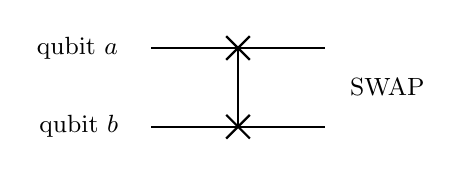
\begin{tikzpicture}[scale=1.0, every node/.style={font=\small}]
  \node[left] at (-0.3,1.5) {qubit $a$};
  \node[left] at (-0.3,0.5) {qubit $b$};
  \draw[thick] (0,1.5) -- (2.2,1.5);
  \draw[thick] (0,0.5) -- (2.2,0.5);
  \draw[thick] (0.95,1.35) -- (1.25,1.65);
  \draw[thick] (0.95,1.65) -- (1.25,1.35);
  \draw[thick] (0.95,0.35) -- (1.25,0.65);
  \draw[thick] (0.95,0.65) -- (1.25,0.35);
  \draw[thick] (1.1,1.5) -- (1.1,0.5);
  \node[right] at (2.4,1.0) {SWAP};
\end{tikzpicture}
\caption{Symbolic SWAP gate: the two crosses joined by a vertical line exchange the states of the two qubits. When the hardware lacks a direct connection between the qubits, the compiler realizes a SWAP as three CNOT gates, which is why routing inflates CX depth.}
\label{fig:tikz-swap}
\end{figure}

\subsection{What simulators capture and what they omit}
A simulator reveals some things and hides others, and it helps to be explicit about which. Density-matrix simulation with depolarizing channels answers one specific question: \emph{how fragile is the ideal circuit under a simple, memoryless gate-error model?} ``Memoryless'' here (technically \emph{Markovian}) means each gate's error is independent of everything that came before, with no slow drift and no memory of earlier operations. Real hardware is messier and adds several effects on top: \emph{drift} (the calibration sliding out of tune over time), \emph{temporal correlations} (errors that do depend on the recent past), \emph{spectator qubits} and \emph{crosstalk} (idle or neighbouring qubits nudging the ones in use), and \emph{pulse distortion} (the analog control signals not keeping their intended shape). All of these are costly to measure and fold faithfully into a simulator~\cite{Preskill2018NISQ,Geng2023ImprovedFRQI}. The scope here is therefore deliberate: by holding the same noise model fixed across the naive and v-chain preparations, the \emph{paired} comparison isolates the effect of the preparation structure itself instead of chasing device-specific quirks. The practical consequence is that a large simulated fidelity gap should be read as a hypothesis to confirm on real hardware with layout-aware compilation, not as a deployment guarantee.

\section{Multi-controlled gate synthesis}
FRQI preparation compares the position register against each pixel address, applies multi-controlled $X$ patterns, and steers an $R_y$ rotation on the color qubit. The cost of a multi-controlled $X$ depends heavily on whether ancillas are available and on the decomposition used~\cite{Vale2023MCSU2,Azevedo2024LowDepthMCG,Arsoski2024MCXQFT,Zindorf2024EfficientMCG}. Qiskit's \texttt{MCXGate} exposes modes such as \texttt{noancilla} (no clean ancillas, large CX substructure per slice in the worst case) and \texttt{v-chain} (dirty ancillas, more qubits but often lower CX after transpilation). This thesis compares those two engineering modes while keeping the abstract FRQI state fixed.

The essential trade is ancilla qubits against CNOT depth. V-chain constructions are attractive when ancillas can be borrowed from idle workspace, because they shorten the sequential CX chains that dominate error accumulation~\cite{Azevedo2024LowDepthMCG}. Noancilla decompositions avoid widening the Hilbert space but can explode two-qubit counts, which is why this study only fully transpiles them at the smallest image where compilation stays tractable~\cite{Zindorf2024EfficientMCG}. The QFT-based constructions surveyed by Arsoski show that multi-controlled gates are not monolithic and that their best realization can depend on circuit context~\cite{Arsoski2024MCXQFT}; the present scope is narrower, treating the two built-in Qiskit strategies as proxies for ``expensive but compact'' versus ``cheaper but wider.'' \Cref{tab:mcx-scaling} states the informal scaling.

\begin{table}[htbp]
\centering
\caption{Informal asymptotic scaling for FRQI-style preparation.}
\label{tab:mcx-scaling}
\small
\begin{tabular}{p{3.6cm}p{2.4cm}p{2.4cm}p{4.6cm}}
\toprule
Template & Ancillas & Leading CX order & Comment \\
\midrule
Naive \texttt{noancilla} MCX per pixel & none & $\Theta(N_{\mathrm{pix}}\,2^{m})$ with $m{=}2\log_2 N$ & Matches worst-case decompositions of many controlled-$X$ layers~\cite{Zindorf2024EfficientMCG}. \\
V-chain per pixel & $\le m{-}2$ dirty & $\Theta(N_{\mathrm{pix}}\,m)$ & Ancillas buy shorter chains; still linear in pixel count~\cite{Vale2023MCSU2,Azevedo2024LowDepthMCG}. \\
\bottomrule
\end{tabular}
\end{table}

\section{Readout error mitigation}
This section makes the readout-correction idea sketched earlier concrete. Recall that the measurement hardware occasionally reports the wrong bit, and that these mistakes are \emph{systematic}, so they can be measured once and then undone. The bookkeeping device is a small \emph{confusion matrix} $A$. For a single qubit it is $2\times 2$, and the entry in row $i$, column $j$ is the probability that the device \emph{reports} outcome $i$ when the qubit is truly in state $j$:
\begin{equation}
A = \begin{bmatrix} P(0\,|\,0) & P(0\,|\,1) \\[2pt] P(1\,|\,0) & P(1\,|\,1) \end{bmatrix}.
\end{equation}
Since every true state must be reported as \emph{something}, each column adds up to one; a matrix with that property is called \emph{(column-)stochastic}. Its entries are filled in by a one-time \emph{calibration} experiment: prepare a known $\ket{0}$ many times and tally how often each result comes back, then repeat for $\ket{1}$. Writing the true outcome probabilities as a vector $\mathbf{p}$, the frequencies actually observed are the mixed version $\mathbf{p}' = A\mathbf{p}$.

\emph{Mitigation} simply runs this relationship backwards. Solving $\mathbf{p}' = A\mathbf{p}$ for the unknown true probabilities gives $\mathbf{p} = A^{-1}\mathbf{p}'$, which subtracts the systematic bias back out of the measured counts. When the device is noisy, $A$ sits close to having no inverse (it is \emph{ill-conditioned}), and a plain inversion would magnify the ordinary shot-to-shot scatter; adding a small \emph{Tikhonov} term keeps the solution stable at the price of a slight, deliberate bias. This work implements exactly this $2\times 2$ correction on the FRQI color qubit, kept separate from the density-matrix depolarizing study so that the two error sources are not conflated. The arrangement shows cleanly how a mitigation layer would sit \emph{in front of} intensity decoding: correct the color-qubit statistics first, then turn the corrected probabilities back into a grayscale value~\cite{Mu2025GuidedImageFiltering}.

\section{Positioning of this thesis}
In \Cref{tab:positioning} the thesis is being compared with other works based on certain factors.

\begin{table}[htbp]
\centering
\caption{Positioning relative to typical prior work.}
\label{tab:positioning}
\small
\begin{tabular}{p{2.8cm}p{3.5cm}p{3.5cm}p{3.5cm}}
\toprule
Dimension & Surveys / NEQR edge & Hybrid / hardware FRQI & This thesis \\
\midrule
Primary goal & Taxonomy, operators & Device-aware prep & Structural prep only \\
Hardware & Mixed & Superconducting & Simulator (Aer) \\
Noise & Often ideal & Device noise & Depolarizing + readout slice \\
Metrics & Various & Fidelity / app-specific & PSNR, SSIM, edge SSIM, CX \\
\bottomrule
\end{tabular}
\end{table}
